\begin{figure}[tb]
\vspace{-.35in}
\hspace*{-.5in}
\centering
	\begin{center}
		\setlength{\tabcolsep}{1pt}
		%\hspace*{-1.5cm}
		\begin{tabular}{  c | c | c }
\hspace*{-.1in} & \large{\textsf{NO ATM. ERROR}}   &\large{\textsf{ATM. ERROR}}      \\  \hline


& \vspace{-0.05in} & \\

\hspace*{-.1in} \multirow{1}{*}[0.9in]{ \rotatebox[origin=t]{90}{  \large{\textsf{Video 1}} }} & \hspace{0.05in} {{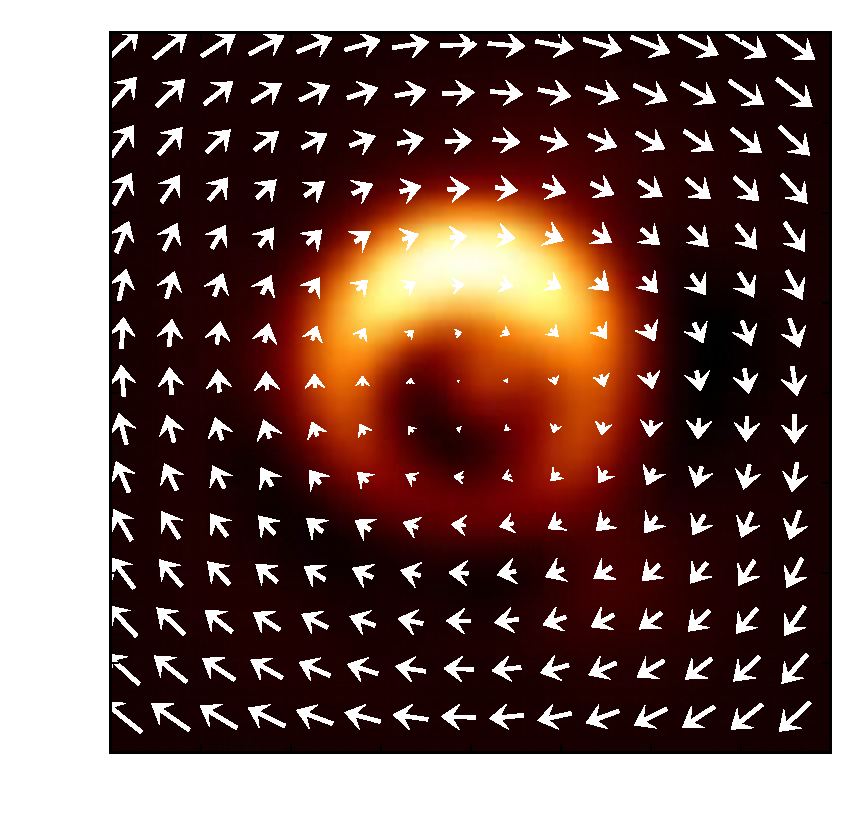
\includegraphics[height=0.35\linewidth]{figures/recov_flowfields/rot30_vis/flow_crop.pdf}} } \hspace{0.005in}  & \hspace{0.05in}
{{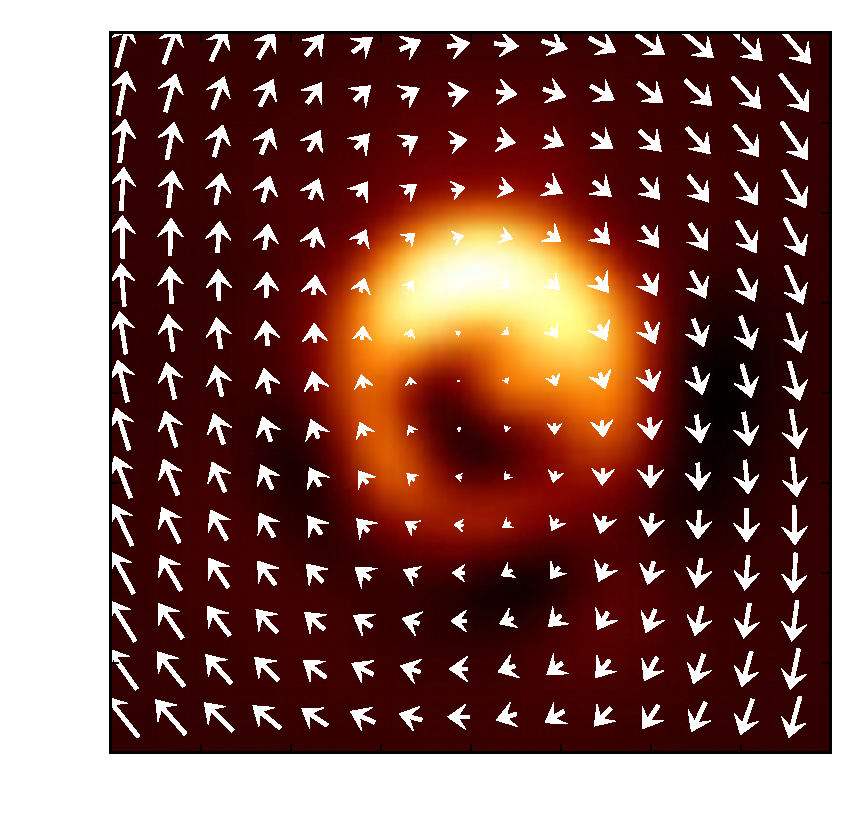
\includegraphics[height=0.35\linewidth]{figures/recov_flowfields/rot30_bis/flow_crop.pdf}} } \\ 

& \vspace{-0.09in} & \\

\hline

& \vspace{-0.05in} & \\

\hspace*{-.1in} \multirow{1}{*}[0.9in]{ \rotatebox[origin=t]{90}{ \large{\textsf{Video 2}} }} \hspace{0.06in}  &  \hspace{0.05in} {{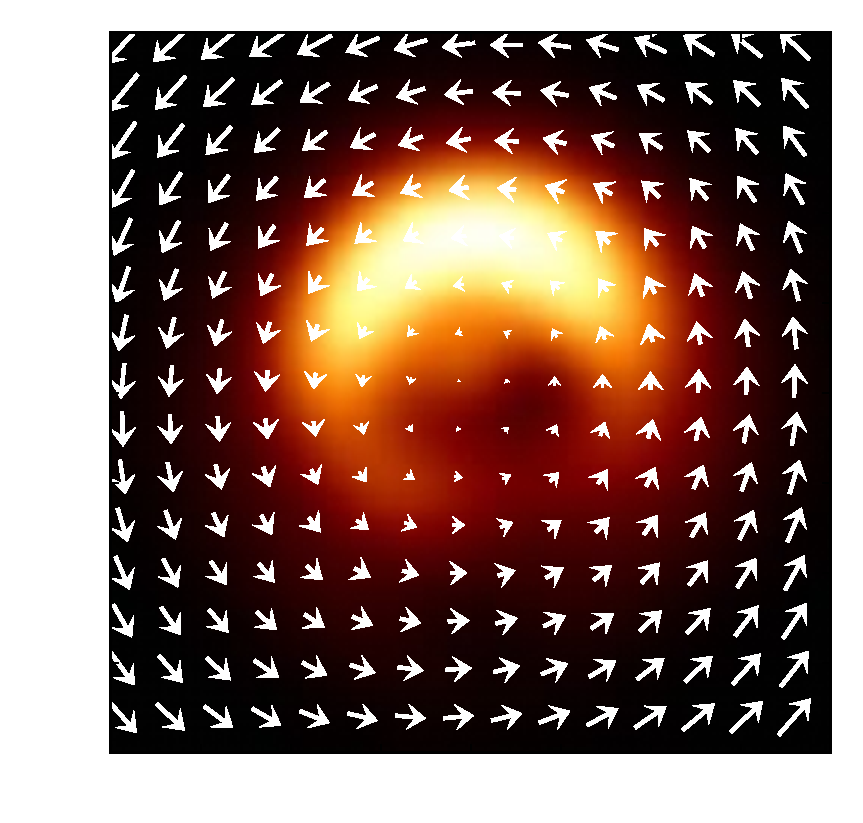
\includegraphics[height=0.35\linewidth]{figures/recov_flowfields/hotspot100sR2_vis/flow_crop.pdf}} }  \hspace{0.005in}& \hspace{0.05in}
{{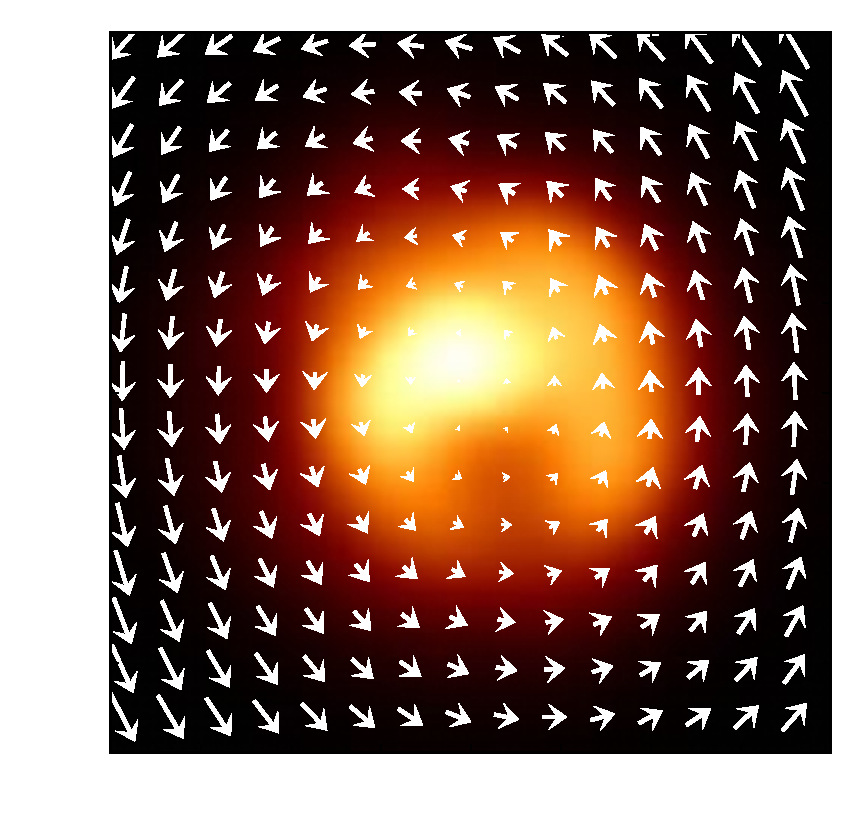
\includegraphics[height=0.35\linewidth]{figures/recov_flowfields/hotspot100sR2_bis/flow_crop.pdf}} }
\end{tabular}
\end{center}
\caption{{\bf Recovering Warp Field:} By solving for the parameters of a persistent warp field using the proposed EM algorithm, we are able to recover a low-dimensional representation of the source dynamics. Results are shown using the EHT2017+ array with and without atmospheric error (ATM. and NO ATM. ERROR, respectively). Arrows showing the direction of recovered motion are overlaid on the mean image for a recovered video. Refer to the supplemental video for a visualization of the true underlying and recovered videos. In Video 1 the true underlying motion can be described by a clockwise rotation. The proposed method is able to recover Video 1's motion from the observed data. Video 2 contains a `hot spot' rotating counter-clockwise around a static emission. Video 2 cannot be described using a single persistent flow field. Yet, despite this, the proposed method is still able to recover the general direction of counter-clockwise motion. 
}
\label{fig:warpfield}
\vspace{-.15in}
\end{figure}